%\setcounter{section}{-1}

\section*{Introduction}\label{sec:Introduction}

Readers will have encountered \emph{peer production}, at least in applications like Wikipedia, StackExchange, and free/libre/open source software development.   
%
Readers will also be familiar with \emph{Peeragogy}, even if the name is unfamiliar.  Simply put, peeragogy is active learning together with others.  Participants in a peeragogical endeavor collaboratively build emergent structures that are responsive to their changing context. They learn -- and they adapt.
% 
Taking inspiration from the notable successes of peer production, we are using peeragogy to help design the future of learning, inside and outside of institutions.

We have found design patterns useful for organizing our work on this momentous task.  However, there is a difference between the pattern language we present here and previous collections of design patterns that touch on similar domains -- like \emph{Liberating Voices: A Pattern Language for Communication Revolution} \cite{schuler2008liberating} and \emph{Pedagogical Patterns: Advice for Educators} \cite{bergin2012pedagogical}.  At the level of the pattern template, our innovation is simply to add a ``What's next'' annotation to each pattern, which anticipates the way the pattern will continue to ``resolve'' in our work. 

% The patterns we introduce here focus on negotiating the execution and implementation of solutions in their practical context.
%  This often requires compromise, adjustments and even restarts.  

This mirrors the central considerations of our approach, which is all about human interaction, and the challenges, fluidity and lack of predictability that comes with it.  Something that works for one person may not work for another or may not even work for the same person in a slightly different situation.  Nevertheless, it is hard to argue with a formula like ``If W applies, do X to get Y.'' In our view, other pattern languages often achieve this sort of common sense rationality, and then stop.  Failure in the prescriptive model only begins when people try to define things more carefully and make context-specific changes -- when they actually try to put ideas into practice.  The problem lies in the inevitable distance between \emph{do as I say}, \emph{do as I do}, and \emph{do with me} \cite[p.~26]{deleuze1994difference}.
%One is put in mind of Alfred Korzybski's famous remark: ``the map is not the territory.''   

This paper outlines a new approach to the organization of learning, drawing on the principles of free/libre/open source software (FLOSS) and open culture.  Mako Hill suggests that one recipe for success in peer production is to take a familiar idea -- his example is an encyclopedia -- and make it easy for people to participate in building it \cite[Chapter 1]{mako-thesis}.  Another inspiring familiar idea is the university.  We will take hold of ``learning in institutions'' as a map (Figure \ref{madison-map}), though it does not fully conform to the tacitly-familiar territory of peeragogy.  To be clear, peeragogy is not just for teachers and students, but for \emph{any group of people who want to learn anything}.\footnote{\url{https://www.youtube.com/watch?v=TDRGJzoNbAc}}

\begin{wrapfigure}{l}{.52\textwidth}
\vspace{-.9cm}
\begin{center}
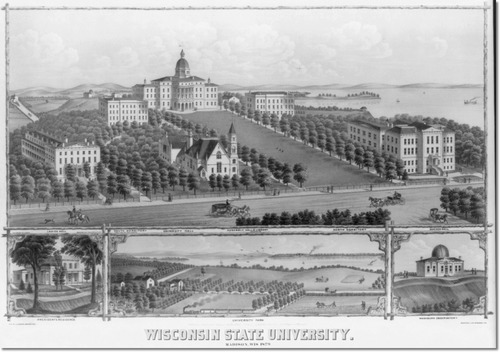
\includegraphics[width=.5\textwidth,trim=0 30 10 2, clip=true]{wisconsin-map}
\end{center}
\vspace{-.1cm}
\caption{A prototypical university.  Caption reads: ``Wisconsin State
  University, Madison, Wis. 1879''.  Inset captions describe the
  pictured buildings: ``Ladies Hall, South Dormitory, University Hall,
  Assembly Halls \& Library, North Dormitory, Science Hall, President's
  Residence, University Farm, and Washburn Observatory.''  Public
  domain.\label{madison-map}}
\vspace{-.6cm}
\end{wrapfigure}

%OSS: Change abstract to free culture 
%OSS: New apporach? Put some things together that are not together elsewhere? Have an order and new look into this process
This paper outlines a new approach to the organization of learning, drawing on the principles of free/libre/open source software (FLOSS) and open culture.  Mako Hill suggests that one recipe for success in peer production is to take a familiar idea -- his example is an encyclopedia -- and make it easy for people to participate in building it \cite[Chapter 1]{mako-thesis}.  Another inspiring familiar idea is the university.  We will take hold of ``learning in institutions'' as a map (Figure \ref{madison-map}), though it does not fully conform to the tacitly-familiar territory of peeragogy.  To be clear, peeragogy is not just for teachers and students, but for \emph{any group of people who want to learn anything}.\footnote{\url{https://www.youtube.com/watch?v=TDRGJzoNbAc}}

%% Indeed, the strong version of our claim is that peeragogy is needed in applications of any map, blueprint, or design that seeks to involve people as people.
In some idealized sense, ``control'' is all that's required to move from a well-thought-out design to successful execution.  But, at the very least, this leaves the question: where do the designs come from in the first place \cite{von2003cybernetics}?
%
Once they exist, designs need to be interpreted, and often, revised.  Many designs need to involve people as people; and people may think that they are on the same page, only to find out that their understandings are wildly different.  For  example, everyone may agree that the group needs to go ``that way.''  But how far?  How fast?  It is rare for a project to be able to set or even define all parameters accurately and concisely at the beginning.

This is true for pattern languages as well.  We describe them in text, but they become a ``living language'' \cite[p.~xvii]{alexander1977pattern}  just insofar as they are linked to action.  Many things have changed since Alexander suggested that ``you will get the most `power' over the language, and make it your own most effectively, if you write the changes in, at the appropriate places in the book'' \cite[p.~xl]{alexander1977pattern}.  We see more clearly that we can build living designs, and inscribe their changing form not just in the margins of a book, or even a shared wiki, but in the lifeworld itself.  

Although we are often thinking about learning and adaptation that takes
place far outside of formal institutions, the historical conception
of the university can offer some guidance.
%
The model university is not separate from the life of the state or its
citizenry, but aims to ``assume leadership in the application of
knowledge for the direct improvement of the life of the people in
every sphere'' \cite[p.~88]{curti1949university}. Research that \emph{adds
to the store of knowledge} is another fundamental
obligation \cite[p.~550]{curti1949university}.    
%% We use the patterns of peeragogy to
%% \emph{constitute and occupy practical or speculative problems as such}
%% \cite[p.~204]{deleuze1994difference}.
%% %
%% Our patterns are a living language just insofar as they are linked to
%% action.

% Till Sch{\"u}mmer \emph{et al.}~have emphasized that pattern authors ``talk about what by definition is tacit'' and highlight the role of nonverbal communication ``needed to communicate the unspeakable'' \cite[p.~9]{schummer2014beyond}.

Our emergent approach to collaboration and knowledge-building is likely to be of interest to theorists in fields like organization studies and, perhaps surprisingly, computer science, where researchers are increasingly making use of social approaches to software design and development (e.g., via the \href{http://www.agilemanifesto.org/}{Manifesto for Agile Software Development}) as well as agent-based models of computation and learning \cite{minsky1967programming,poetry-workshop}.  
%
The design pattern community in particular is very familiar with practices that we think of as peeragogical, notably shepherding and writers workshops \cite{harrison1999language,coplien1997pattern}.  We hope to help design pattern authors and researchers expand on these strengths.

\subsection*{Plan of the work}

\begin{wraptable}{r}{.52\textwidth}
\vspace{-.10cm}
\begin{tabular}{|p{.5\textwidth}|}
\hline
\emph{Motivation} for using this pattern.\\ \hline
\emph{Context} of application.\\ \hline
\emph{Forces} that operate within the context of application. \\ \hline
\emph{Problem} the pattern addresses.\\ \hline
\emph{Solution} to the problem.\\ \hline
\emph{Rationale} for this solution.\\ \hline
\emph{Resolution} of the forces.\\ \hline
\emph{Example 1}: How the pattern manifests in current Wikimedia projects.\\ \hline
\emph{Example 2}: How the pattern could inform the design of a future university.\\ \hline
``\emph{What's Next}'': Our collective intention in the Peeragogy project\\ \hline
\end{tabular}
\vspace{-.1cm}
\caption{Pattern template.\label{tab:pattern-template}}
\vspace{-.6cm}
\end{wraptable}

This section is intended to give the reader an idea of how the paper is organized. Section \ref{sec:Peeragogy} explains the concept of \patternname{Peeragogy} explicitly in the form of a design pattern. Sections \ref{sec:Roadmap}--\ref{sec:Scrapbook} present the other patterns in our pattern language. Figure \ref{fig:connections} illustrates their interconnections.

Table \ref{tab:pattern-template} shows the pattern template that we use throughout the paper.  Each pattern includes two illustrative examples.  The first is descriptive, and looks at how the pattern applise in current Wikimedia projects.  The second is prospecttive and shows show how the pattern could be applied in the design of a future university.  Whereas existing projects like Wikimedia's Wikiversity\footnote{\url{https://www.wikiversity.org/}} and the Peer-2-Peer University (P2PU) have created ``a model for lifelong learning alongside traditional formal higher education,''\footnote{\url{https://www.p2pu.org/en/}} they stop well short of offering accredited degrees.  What would an accredited free/libre/open university offering general education look like?  How would it compare or contrast with the typical or stereotypical image of a university from Figure \ref{madison-map}?
Each pattern concludes with a boxed ``\emph{What's Next}'' annotation that is specific to our collective intention in the Peeragogy project.

Section \ref{sec:Distributed_Roadmap} collects these next steps and summarizes the outlook of the Peeragogy project.  Section \ref{sec:Conclusion} reviews the contributions made in the paper, positioning this work as a hands-on complement to existing sociological and historical research about peer production (surveyed in \cite{benkler2015peer}).

%OSS: who cares? start w/example?
\subsection*{A short motivating example}
When one relative \patternname{Newcomer} was still in the onboarding process in Peeragogy Project, she hit a wall in understanding the ``patterns'' section in the Peeragogy Handbook v1. A more seasoned peer invited her to a series of separate sessions to flesh out the patterns and make them more accessible to newcomers. During those sessions, the impact and meaning of patterns captured her imagination. She continued on to become the champion for pattern language and application in the Project, helped revise the pattern language section for v3, and attended PLoP 2015. While it can easily get overwhelming, this newcomer found \patternname{A specific project} to start and scaffolded her knowledge and contributions from that base.

\begin{figure}
\vspace{-.9in}
{\centering
\begin{tikzpicture}[dot/.style={circle,inner sep=1pt,fill,name=#1}]
%\draw[step=1cm,gray,very thin] (0,0) grid (10,10);
\node (assess) at (5, 9.75) {{\Large {\sc Assess}}};
\node (organize) at (5, 0) {{\Large {\sc Organize}}};
\node (cooperate)[text width=2cm,align=center,rotate=270] at (10, 5) {{\Large {\sc Convene}}};
\node (convene)[text width=15cm,align=center,rotate=90] at (0, 5) {{\Large {\sc Cooperate}}};

\node(legend)[draw,rectangle,text width=2.67cm] at (9.25,.75) 
{\begin{tabular}{p{2.7cm}@{\hspace{-1mm}}}
\textbf{Legend}\\ \hline\vspace{-2mm} \textbf{A}\hspace{.41in}\textbf{B}\\
if pattern \textbf{A} refers to pattern \textbf{B}.
  \end{tabular}};
\draw[-{Latex[width=2mm]},draw=gray] ([xshift=5mm,yshift=1.75mm]legend.west) -- ([xshift=-14.8mm,yshift=1.75mm]legend.east);

%%%%%%%%%%%%%%%%%%%%%%%%%%%%%%%%%%%%%%%%%%%%%%%%%%%%%%%%%%%%%%%%%%%%%%%%%%%%%%%%%%%%%%%%%%%%%%%%%%%%%
\node[below = 5cm of assess] (roadmap) {\ref{sec:Roadmap}. \hyperref[sec:Roadmap]{\emph{Roadmap}}};
\node (reduce) at (5, 8.75) {\ref{sec:Reduce, reuse, recycle}. \hyperref[sec:Reduce, reuse, recycle]{\emph{Reduce, reuse, recycle}}};
\node (carryingcapacity) at (1.25, 7.15) {\ref{sec:Carrying capacity}. \hyperref[sec:Carrying capacity]{\emph{Carrying capacity}}};
\node[below = 3.2cm of carryingcapacity] (heartbeat) {\ref{sec:Heartbeat}. \hyperref[sec:Heartbeat]{\emph{Heartbeat}}};
\node (aspecificproject) at (8.5, 6.5) {\ref{sec:A specific project}. \hyperref[sec:A specific project]{\emph{A specific project}}};
\node[below = 1cm of roadmap] (wrapper) {\ref{sec:Wrapper}. \hyperref[sec:Wrapper]{\emph{Wrapper}}};
\node (newcomer) at (8.5, 3.25) {\ref{sec:Newcomer}. \hyperref[sec:Newcomer]{\emph{Newcomer}}};
\node[below = 1.7cm of wrapper] (scrapbook) {\ref{sec:Scrapbook}. \hyperref[sec:Scrapbook]{\emph{Scrapbook}}};
\node[above = 1cm of aspecificproject] (peeragogyproject) {\ref{sec:Peeragogy}. \hyperref[sec:Peeragogy]{\emph{Peeragogy}}};
%%%%%%%%%%%%%%%%%%%%%%%%%%%%%%%%%%%%%%%%%%%%%%%%%%%%%%%%%%%%%%%%%%%%%%%%%%%%%%%%%%%%%%%%%%%%%%%%%%%%%
\draw[-{Latex[width=2mm]},draw=gray] (peeragogyproject) -- (aspecificproject);
% \draw[-{Latex[width=2mm]},draw=gray] (aspecificproject) -- (par);
\draw[-{Latex[width=2mm]},draw=gray] (aspecificproject) -- (roadmap);
\draw[-{Latex[width=2mm]},draw=gray] (aspecificproject.230) to[out=250,in=40] (scrapbook);
\draw[-{Latex[width=2mm]},draw=gray] (aspecificproject) -- (carryingcapacity);
\draw[-{Latex[width=2mm]},draw=gray] (carryingcapacity.337) -- (newcomer);
\draw[-{Latex[width=2mm]},draw=gray] (carryingcapacity.330) -- (roadmap);
\draw[-{Latex[width=2mm]},draw=gray] (carryingcapacity) -- (peeragogyproject);
\draw[-{Latex[width=2mm]},draw=gray] ([xshift=1mm]carryingcapacity.south) -- (scrapbook.140);
% \draw[-{Latex[width=2mm]},draw=gray] ([xshift=2mm]creatingaguide.160) to[out=-215,in=-67] (carryingcapacity);
\draw[-{Latex[width=2mm]},draw=gray] (heartbeat) -- (aspecificproject.185);
\draw[-{Latex[width=2mm]},draw=gray] (heartbeat) -- (carryingcapacity);
\draw[-{Latex[width=2mm]},draw=gray] (heartbeat) -- (scrapbook.155);
\draw[-{Latex[width=2mm]},draw=gray] (heartbeat) -- (reduce.215);
\draw[-{Latex[width=2mm]},draw=gray] (newcomer) -- ([xshift=4mm]reduce.south);
\draw[-{Latex[width=2mm]},draw=gray] (newcomer) -- (aspecificproject);
% \draw[-{Latex[width=2mm]},draw=gray] (newcomer) -- (creatingaguide.north);
\draw[-{Latex[width=2mm]},draw=gray] (newcomer) -- (roadmap.350);
\draw[-{Latex[width=2mm]},draw=gray] (newcomer) -- (scrapbook.24);
% \draw[-{Latex[width=2mm]},draw=gray] (par) -- (scrapbook);
\draw[-{Latex[width=2mm]},draw=gray] (roadmap) -- (peeragogyproject.195);
\draw[-{Latex[width=2mm]},draw=gray] (roadmap.350) -- (newcomer);
\draw[-{Latex[width=2mm]},draw=gray] (roadmap) -- (wrapper);
\draw[-{Latex[width=2mm]},draw=gray] ([yshift=.3mm]roadmap.west) -- (heartbeat);
\draw[-{Latex[width=2mm]},draw=gray] (roadmap) -- (aspecificproject);
% \draw[-{Latex[width=2mm]},draw=gray] (scrapbook) -- (par);
\draw[-{Latex[width=2mm]},draw=gray] (scrapbook) -- (wrapper);
\draw[-{Latex[width=2mm]},draw=gray] (scrapbook.110) to[out=123,in=250] (reduce.245);
\draw[-{Latex[width=2mm]},draw=gray] (scrapbook.70) to[out=43,in=305] (roadmap.330);
% \draw[-{Latex[width=2mm]},draw=gray] ([xshift=2mm,yshift=-.4mm]reduce.south) -- (creatingaguide);
\draw[-{Latex[width=2mm]},draw=gray] (reduce) -- (carryingcapacity);
\draw[-{Latex[width=2mm]},draw=gray] (reduce) -- (roadmap);
\draw[-{Latex[width=2mm]},draw=gray] ([xshift=.7mm]wrapper.175) -- (heartbeat);
\draw[-{Latex[width=2mm]},draw=gray] ([xshift=-.7mm,yshift=-.3mm]wrapper.360) -- (newcomer);
\draw[-{Latex[width=2mm]},draw=gray] (wrapper) -- ([xshift=2.3mm]carryingcapacity.south);
\draw[-{Latex[width=2mm]},draw=gray] (wrapper) -- (roadmap);

\end{tikzpicture}


\par
}
\vspace{-.9in}
\caption{Connections between the patterns of peeragogy.  An arrow points from pattern \textbf{A} to pattern \textbf{B} if the text of the description of pattern \textbf{A} references pattern \textbf{B}.  Labels at the borders of the figure correspond to the main sections of the \emph{Peeragogy Handbook}.\label{fig:connections}}
\end{figure}

\begin{table}
{\footnotesize
\begin{tabular}{|p{\textwidth}|}
\hline
\rowcolor{Gray!30} \multicolumn{1}{|l|}{\color{Black} \ref{sec:Peeragogy}. \patternname{Peeragogy}: \textbf{How can we solve problems together?}}\\
\hline
\vspace{.01em}
\begin{minipage}{\textwidth}
\begin{description}
\item[$\leftarrow$\patternname{Roadmap}] We need to figure out how to get from ``here'' to ``there''.
\item[$\leftarrow$\patternname{Carrying capacity}] Each contributor has bounded time and other resources.
\end{description}
\end{minipage}
\vspace{.25em}\\
\hline 
%%%%%%%%%%%%%%%%%%%%
\rowcolor{Gray!30} \multicolumn{1}{|l|}{\color{Black} \ref{sec:Roadmap}. \patternname{Roadmap}: \textbf{How can we keep track of what everyone is doing?}}\\
\hline
\vspace{.01em}
\begin{minipage}{\textwidth}
\begin{description}
\item[$\leftarrow$\patternname{Reduce, reuse, recycle}] A plan develops by making sense of existing resources.
\item[$\leftarrow$\patternname{Carrying capacity}] As difficulties are encountered the plan should be revised.
\item[$\leftarrow$\patternname{A specific project}] The project may cover many connected sub-projects.
\item[$\leftarrow$\patternname{Wrapper}] Someone in the project needs to make sure the plan reflects reality.
\item[$\leftarrow$\patternname{Newcomer}] If new participants have trouble getting involved, the plan should be revised.
\end{description}
\end{minipage}
\vspace{.25em}\\
\hline
%%%%%%%%%%%%%%%%%%%%
\rowcolor{Gray!30} \multicolumn{1}{|l|}{\color{Black} \ref{sec:Reduce, reuse, recycle}. \patternname{Reduce, reuse, recycle}: \textbf{How can we avoid undue isolation?}}\\
\hline
\vspace{.01em}
\begin{minipage}{\textwidth}
\begin{description}
\item[$\leftarrow$\patternname{Heartbeat}] As we notice new spin-off or spin-in projects, we can give them energy.
\item[$\leftarrow$\patternname{Newcomer}] Each potential contributor brings a somewhat new approach.
\item[$\leftarrow$\patternname{Scrapbook}] We can keep track of great ideas coming from many different sources.
\end{description}
\end{minipage}
\vspace{.25em}\\
\hline
%%%%%%%%%%%%%%%%%%%%
\rowcolor{Gray!30} \multicolumn{1}{|l|}{\color{Black} \ref{sec:Carrying capacity}. \patternname{Carrying capacity}: \textbf{How can we avoid becoming overwhelmed?}}\\
\hline
\vspace{.01em}
\begin{minipage}{\textwidth}
\begin{description}
%%% Revise here
\item[$\leftarrow$\patternname{Reduce, reuse, recycle}] All available perspectives are useful for the project.
\item[$\leftarrow$\patternname{A specific project}] We may need help to create or activate a plan.
\item[$\leftarrow$\patternname{Wrapper}] Share skills and be transparent about limitations and bottlenecks.
\item[$\leftarrow$\patternname{Heartbeat}] Project activites should give us rewards, not drain our energy.
\end{description}
\end{minipage}
\vspace{.25em}\\
\hline
%%%%%%%%%%%%%%%%%%%%
\rowcolor{Gray!30} \multicolumn{1}{|l|}{\color{Black} \ref{sec:A specific project}. \patternname{A specific project}: \textbf{How can we avoid becoming perplexed?}}\\
\hline
\vspace{.01em}
\begin{minipage}{\textwidth}
\begin{description}
\item[$\leftarrow$\patternname{Peeragogy}] We can collaborate on (the intersections of) specific projects.
\item[$\leftarrow$\patternname{Roadmap}] In some cases we can lay out the potential tasks far in advance.
\item[$\leftarrow$\patternname{Heartbeat}] We may alternate open discussion with focused work sessions.
\item[$\leftarrow$\patternname{Newcomer}]As we find our way from motivation to action, we add concreteness.
\end{description}
\end{minipage}
\vspace{.25em}\\
\hline
%%%%%%%%%%%%%%%%%%%%
\rowcolor{Gray!30} \multicolumn{1}{|l|}{\color{Black} \ref{sec:Wrapper}. \patternname{Wrapper}: \textbf{How can people stay in touch with the project?}}\\
\hline
\vspace{.01em}
\begin{minipage}{\textwidth}
\begin{description}
\item[$\leftarrow$\patternname{Roadmap}]If project participants are not all contributing, someone may take charge.
\item[$\leftarrow$\patternname{Scrapbook}] One part of this responsible role is to gather outstanding concerns.
\end{description}
\end{minipage}
\vspace{.25em}\\
\hline
%%%%%%%%%%%%%%%%%%%%
\rowcolor{Gray!30} \multicolumn{1}{|l|}{\color{Black} \ref{sec:Heartbeat}. \patternname{Heartbeat}: \textbf{How can we make the project ``real'' for participants?}}\\
\hline
\vspace{.01em}
\begin{minipage}{\textwidth}
\begin{description}
\item[$\leftarrow$\patternname{Roadmap}] The simplest plan may just be to meet together from time to time.
\item[$\leftarrow$\patternname{Wrapper}] It can be useful to set things up so that people can follow different rhythms.
\end{description}
\end{minipage}
\vspace{.25em}\\
\hline
%%%%%%%%%%%%%%%%%%%%
\rowcolor{Gray!30} \multicolumn{1}{|l|}{\color{Black} \ref{sec:Newcomer}. \patternname{Newcomer}: \textbf{How can we make the project accessible to new people?}}\\
\hline
\vspace{.01em}
\begin{minipage}{\textwidth}
\begin{description}
\item[$\leftarrow$\patternname{Roadmap}] Transparency can show outsiders what it would be like to get involved.
\item[$\leftarrow$\patternname{Carrying capacity}] Boosting the project's capacity may require training in new participants.
\item[$\leftarrow$\patternname{Wrapper}] Ideally we would actively welcome all contributions with love.
\end{description}
\end{minipage}
\vspace{.25em}\\
\hline
%%%%%%%%%%%%%%%%%%%%
\rowcolor{Gray!30} \multicolumn{1}{|l|}{\color{Black} \ref{sec:Scrapbook}. \patternname{Scrapbook}: \textbf{How can we maintain focus as time goes by?}}\\
\hline
\vspace{.01em}
\begin{minipage}{\textwidth}
\begin{description}
\item[$\leftarrow$\patternname{Carrying capacity}] It is useful to record obstacles and outstanding challenges.
\item[$\leftarrow$\patternname{A specific project}] We want to stay connected to concrete action, not just theory.
\item[$\leftarrow$\patternname{Heartbeat}] A project that is no longer rewarding may be put on the back burner.
\end{description}
\end{minipage}
\vspace{.25em}\\
\hline

\end{tabular}
}
\caption{Backwards links specify the ``larger'' context for each of our patterns.  This helps to explain the core problem that each pattern in our pattern language addresses. This table records each instance of \textbf{B}$\leftarrow$\textbf{A} where pattern \textbf{A} refers to pattern \textbf{B}.  }
\end{table}

\begin{table}
{\footnotesize
\begin{tabular}{|p{\textwidth}|}
\hline
\rowcolor{Gray!30} \multicolumn{1}{|l|}{\color{Black} \ref{sec:Peeragogy}. \patternname{Peeragogy}: \textbf{Get really concrete about what the problems are.}}\\
\hline
\vspace{.01em}
\begin{minipage}{\textwidth}
\begin{description}
\item[$\rightarrow$\patternname{A specific project}] The way to make progress is to get specific.
\end{description}
\end{minipage}
\vspace{-.05em}\\
\hline 
%%%%%%%%%%%%%%%%%%%%
\rowcolor{Gray!30} \multicolumn{1}{|l|}{\color{Black} \ref{sec:Roadmap}. \patternname{Roadmap}: \textbf{Build a plan that we keep updating as we go along.}}\\
\hline
\vspace{.01em}
\begin{minipage}{\textwidth}
\begin{description}
\item[$\rightarrow$\patternname{A specific project}] The project shouldn't solve all problems.
\item[$\rightarrow$\patternname{Heartbeat}] People will meet in some rhythm.
\item[$\rightarrow$\patternname{Wrapper}] Someone should help those who are less involved keep apprised of progress.
\item[$\rightarrow$\patternname{Newcomer}] A good plan can help new people get involved.
\end{description}
\end{minipage}
\vspace{.25em}\\
\hline
%%%%%%%%%%%%%%%%%%%%
\rowcolor{Gray!30} \multicolumn{1}{|l|}{\color{Black} \ref{sec:Reduce, reuse, recycle}. \patternname{Reduce, reuse, recycle}: \textbf{Use what's there and share what we make.}}\\
\hline
\vspace{.01em}
\begin{minipage}{\textwidth}
\begin{description}
\item[$\rightarrow$\patternname{Roadmap}] Develop a plan to make sense of existing resources.
\item[$\rightarrow$\patternname{Carrying capacity}] Existing stresses are one resource that we can use.
\end{description}
\end{minipage}
\vspace{.25em}\\
\hline
%%%%%%%%%%%%%%%%%%%%
\rowcolor{Gray!30} \multicolumn{1}{|l|}{\color{Black} \ref{sec:Carrying capacity}. \patternname{Carrying capacity}: \textbf{Clearly express when we're frustrated.}}\\
\hline
\vspace{.01em}
\begin{minipage}{\textwidth}
\begin{description}
%%% Revise here
\item[$\rightarrow$\patternname{Roadmap}] When problems and difficulties are made explicit they can eventually be addressed.
\item[$\rightarrow$\patternname{Newcomer}] If there is too much work to do, finding people to help may be helpful.
\end{description}
\end{minipage}
\vspace{.25em}\\
\hline
%%%%%%%%%%%%%%%%%%%%
\rowcolor{Gray!30} \multicolumn{1}{|l|}{\color{Black} \ref{sec:A specific project}. \patternname{A specific project}: \textbf{Focus on concrete, doable tasks.}}\\
\hline
\vspace{.01em}
\begin{minipage}{\textwidth}
\begin{description}
\item[$\rightarrow$\patternname{Roadmap}] Make your project even more specific by creating a concrete plan.
\item[$\rightarrow$\patternname{Carrying capacity}] Make the scope of the project match your available energy.
\item[$\rightarrow$\patternname{Scrapbook}] Make note of anything you haven't been able to solve and move on.
\end{description}
\end{minipage}
\vspace{.25em}\\
\hline
%%%%%%%%%%%%%%%%%%%%
\rowcolor{Gray!30} \multicolumn{1}{|l|}{\color{Black} \ref{sec:Wrapper}. \patternname{Wrapper}: \textbf{Maintain a coherent public surface.}}\\
\hline
\vspace{.01em}
\begin{minipage}{\textwidth}
\begin{description}
\item[$\rightarrow$\patternname{Roadmap}] Part of your job is to draw out goals and methods that people are using.
\item[$\rightarrow$\patternname{Carrying capacity}] Make note of difficulties that the group encounters.
\item[$\rightarrow$\patternname{Newcomer}] Make the project accessible to newcomers.
\item[$\rightarrow$\patternname{Heartbeat}] Make sure that meetings happen and that reports on those meetings go to the right people.
\end{description}
\end{minipage}
\vspace{.25em}\\
\hline
%%%%%%%%%%%%%%%%%%%%
\rowcolor{Gray!30} \multicolumn{1}{|l|}{\color{Black} \ref{sec:Heartbeat}. \patternname{Heartbeat}: \textbf{Keep up a regular, sustaining rhythm.}}\\
\hline
\vspace{.01em}
\begin{minipage}{\textwidth}
\begin{description}
\item[$\rightarrow$\patternname{Reduce, reuse, recycle}] You can set up spin-off projects when something gets interesting.
\item[$\rightarrow$\patternname{Carrying capacity}] The group should nurture the people in the group.
\item[$\rightarrow$\patternname{A specific project}] Set up regular meetings to focus on specific tasks.
\item[$\rightarrow$\patternname{Scrapbook}] Wind down projects that are no longer helpful.
\end{description}
\end{minipage}
\vspace{.25em}\\
\hline
%%%%%%%%%%%%%%%%%%%%
\rowcolor{Gray!30} \multicolumn{1}{|l|}{\color{Black} \ref{sec:Newcomer}. \patternname{Newcomer}: \textbf{Let's learn from newcomers.}}\\
\hline
\vspace{.01em}
\begin{minipage}{\textwidth}
\begin{description}
\item[$\rightarrow$\patternname{Roadmap}] A new person can give feedback on how clear the plan is.
\item[$\rightarrow$\patternname{A specific project}] Newcomers should adapt their general interest to a specific task.
\end{description}
\end{minipage}
\vspace{.25em}\\
\hline
%%%%%%%%%%%%%%%%%%%%
\rowcolor{Gray!30} \multicolumn{1}{|l|}{\color{Black} \ref{sec:Scrapbook}. \patternname{Scrapbook}: \textbf{Move things that are not of immediate use out of focus.}}\\
\hline
\vspace{.01em}
\begin{minipage}{\textwidth}
\begin{description}
\item[$\rightarrow$\patternname{Roadmap}] Just as we keep track of the future plans, we should also keep track of past events.
\item[$\rightarrow$\patternname{Reduce, reuse, recycle}] Something that is not interesting right now may become interesting later.
\end{description}
\end{minipage}
\vspace{.25em}\\
\hline

\end{tabular}
}
\caption{Forward links specify the ``smaller'' context for each of our patterns.  This helps to explain the core solution that each pattern in our pattern language offers. This table records each instance of \textbf{A}$\rightarrow$\textbf{B} where pattern \textbf{A} refers to pattern \textbf{B}.}
\end{table}

% deferring a more detailed elaboration of next steps in the educational arena to future work that will build on this basis.
% Technology has come a long way since Alexander suggested ``you will get the most `power' over the language, and make it your own most effectively, if you write the changes in, at the appropriate places in the book'' \cite[p.~xl]{alexander1977pattern}.
% While Christian Kohls insightfully describes patterns as the unique resolution of the dynamical forces acting in a given context \cite{kohls2010structure,kohls2011structure}.
%%% Patterns come to you through mindful awareness ... Charlotte: I think about patterns all the time now, I think about what makes me productive in a team.
% So, while we speak the same language as other developers of design patterns, our orientation is somewhat different, and our understanding of the word `pattern' is nuanced because we aim to take full account of the lifecycle of patterns.  Our work contributes to a recent ``performative'' turn \cite{schummer2014beyond}, which we believe gets at the heart of what design patterns can do.
%  
% In practical terms, we believe the patterns that we introduce here will be useful for students and educators who want their work to have real-world relevance, to activists and policy-makers who want to develop practicable solutions to large-scale problems, and to employees and managers who, like it or not, find themselves working in distributed teams. 

  
